\documentclass[a4paper,utf8]{article}
\usepackage[heading,fancyhdr]{ctex}
\usepackage{amsmath,amssymb,geometry,lastpage,ulem}
\usepackage{array,tabularx,tabulary,mhchem,xspace}
\usepackage{floatrow,subfig,multirow,bigstrut}
\usepackage{siunitx,booktabs,longtable,graphicx,xfrac,nameref}
\lineskiplimit=1pt
\lineskip=3pt
\geometry{
    top=25.4mm, 
    left=25mm, 
    right=25mm, 
    bottom=25mm,
    headsep=5.9mm,
}
\ctexset{
    section = {format+=\raggedright}
}
\newcommand{\fgref}[1]{图~\ref{#1}\xspace}
\newcommand{\seqref}[1]{式~(\ref{#1})}
\newcommand{\expinfo}[7][无]{
    {\zihao{-3}\bfseries\songti
    实验名称:\uline{\hfill\mbox{#2}\hfill} \\[2.9mm]
    学\quad 号:\uline{\makebox[25mm]{#3}}\hfill
    姓\quad 名:\uline{\makebox[25mm]{#4}}\hfill
    班\quad 级:\uline{\makebox[25mm]{#5}} \\[2.9mm]
    合作者:\uline{\makebox[25mm]{#1}} \hfill
    桌\quad 号:\uline{\makebox[25mm]{#6}}\hfill\makebox[25mm+4em]{}\\[2.9mm]
    实验日期:\uline{\makebox[30mm]{#7}}\hfill\mbox{} \\[58.7mm]
    }
}
\newcommand{\pointingbox}{
    {\zihao{4}\bfseries\songti%
    实验考核\\[3mm]
    \extrarowheight=3mm
    \begin{tabularx}{150mm}{|X|X|X|X|X|}\hline
        \hfil 项目 \hfil  & \hfil 实验预习 \hfil & \hfil 实验过程 \hfil & \hfil 分析与讨论 \hfil & \hfil 总评 \hfil \\[3mm] \hline
        \hfil 评价 \hfil &  &  &  &  \\[3mm] \hline
    \end{tabularx}
    }
}
\newcommand{\derivative}[2]{\frac{\mathrm{d} #1}{\mathrm{d} #2}}
\newcommand{\thinking}[2]{\textbf{#1}\\
答:\begin{minipage}[t]{0.85\textwidth}
    #2
\end{minipage}}
\pagestyle{fancy}
\fancyhf{} \fancyhead[C]{电路基础实验} \fancyfoot[C]{\thepage~/~\pageref{LastPage}}
\newcounter{Rownumber}
\newcommand*{\Rown}{\stepcounter{Rownumber}\theRownumber}
\newcommand*{\resetRown}{\setcounter{Rownumber}{0}}
\newcommand{\qrange}[3]{\qtyrange[range-phrase = \text{$\sim$},range-units =single]{#1}{#2}{#3}}
\floatsetup[table]{capposition=top}
\newcolumntype{C}{>{\hfil}X<{\hfil}}
\renewcommand{\Nameref}[1]{\textbf{\ref{#1}~\nameref{#1}}} %导入导言
\ctikzset{
    resistors/scale=0.7,
    diodes/scale=0.6}
\begin{document}
\begin{center}
    {\mbox{}\\[7em]\zihao{2}\bfseries\songti%
    电路基础实验报告}\\[34mm]
    \expinfo[王慷]{一阶电路动态过程的研究}{22301056}{王俊杰}{22 材物}{27}{2024.6.4}
\end{center}
\newpage
\section{实验目的}
\begin{enumerate}
    \item 研究一阶电路的零输入响应,零状态响应及全响应的基本规律和特点。
    \item 学习一阶电路时间常数 $\tau$ 的测量方法。
    \item 熟悉微分和积分电路结构,加深对构成微分和积分电路必要条件的理解。
    \item 熟悉示波器的使用方法。
\end{enumerate}

\section{实验原理}%简单描述,含必要的公式和附图;
含有 L、C 元件的电路称动态电路。描述动态电路的方程是微分方程,由给定的初始条件可求得电路的响应。对线性电路其响应可分为零状态响应、零输入响应及全响应。初始状态为零,仅激励引起的响应叫零状态响应;激励为零,由初始条件引起的响应叫零输入响应;同时同激励和初始条件引起的响应叫全响应。电路中只含有一个电感或电容元件时称为一阶电路。\par
一阶电路的零输入响应总是按指数规律衰减,零状态响应总是按指数规律递增或递减,衰减和递增速率的快慢,决定于电路本身参数所确定的时间常数 $\tau$。在 RC 电路中,$\tau=RC$;在 RC 电路中,$\tau=L/R$。\par
动态电路的过渡过程是短暂的单次变化过程,在瞬间发生又很快消失,所以观察这一过程是有困难的,常用方法是用方波仪记录其过程。在实验室中,根据电路时间常数 $\tau$ 的大小不同分别采用不同的实验方法。当 $\tau$ 较大时(数秒),一般采用卡秒表的方法,即在“换路”的同时,既观测电压(或电流)的数值,又启动秒表记录时间,从而可以记录下电压(或电流)随时间变化的规律。当 $\tau$ 较小时,一般采用示波器观测。为了便于观测,必须使单次过渡过程重复出现。可以用方波的前沿代替单次接通直流电源,这样,在方波的每一个前沿和后沿,都出现一次过渡过程。\par
微分电路和积分电路是脉冲数字电路中最常见的波形变换电路。如果输入是方波信号,对于微分电路,当电路时间常数 $\tau$ 远远小于方波的脉冲宽度 $T_\text{p}$(20 倍以上)时,电路输出与输入近似呈微分关系,即将方波变换成正负极性的尖脉冲;对于积分电路,如果电路时间常数 $\tau$ 远远大于方波的脉冲宽度 $T_\text{p}$(20 倍以上),电路输出与输入近似呈积分关系,即将方波变换成三角波。

\section{实验仪表}
    RIGOL MSO2202A 示波器、电路分析实验箱、导线若干。
\section{实验内容与结果}
\subsection{微分电路}
    \begin{figure}[!ht]
        \subfloat[RC 微分电路图\label{fig:1a}]{\includegraphics[width=0.4\textwidth]{1a.png}}\hspace{6mm}
        \subfloat[RL 微分电路图\label{fig:1b}]{\includegraphics[width=0.4\textwidth]{1b.png}}
        \caption{微分电路图}
    \end{figure}
    \subsubsection{RC 微分电路}
        RC 微分电路如图~\ref{fig:1a} 所示,调节方波仪输出频率,使方波脉冲宽度满足微分电路的必要条件,将 $R_2$、$R_4$ 分别接入,观察微分电路输出有何不同,并将波形画在附表中。
        \begin{figure}[!ht]
            \subfloat[$R_2$\label{fig:rcd1}]{\includegraphics[width=0.4\textwidth]{rc_d1.jpg}}\hspace{6mm}
            \subfloat[$R_4$\label{fig:rcd2}]{\includegraphics[width=0.4\textwidth]{rc_d2.jpg}}
            \caption{RC 微分波形图}
        \end{figure}
    \subsubsection{RL 微分电路}
        RL 微分电路如图~\ref{fig:1b} 所示,调节方波仪输出频率,使方波脉冲宽度满足微分电路的必要条件,将 $R_1$、$R_3$ 分别接入,观察微分电路输出有何不同,并将波形画在附表中。
        \begin{figure}[!ht]
            \subfloat[$R_1$\label{fig:rld1}]{\includegraphics[width=0.4\textwidth]{rl_d2.jpg}}\hspace{6mm}
            \subfloat[$R_3$\label{fig:rld2}]{\includegraphics[width=0.4\textwidth]{rl_d1.jpg}}
            \caption{RL 微分波形图}
        \end{figure}
\subsection{积分电路}
    \begin{figure}[!ht]
        \subfloat[RC 积分电路图\label{fig:4a}]{\includegraphics[width=0.4\textwidth]{4a.png}}\hspace{6mm}
        \subfloat[RL 积分电路图\label{fig:4b}]{\includegraphics[width=0.4\textwidth]{4b.png}}
        \caption{微分电路图}
    \end{figure}
    \subsubsection{RC 积分电路}
        RC 积分电路如图~\ref{fig:4a} 所示,调节方波仪输出频率,使方波脉冲宽度满足微分电路的必要条件,将 $R_1$、$R_3$ 分别接入,观察微分电路输出有何不同,并将波形画在附表中。
        \begin{figure}[!ht]
            \subfloat[$R_1$\label{fig:rci1}]{\includegraphics[width=0.4\textwidth]{rc_i1.jpg}}\hspace{6mm}
            \subfloat[$R_3$\label{fig:rci2}]{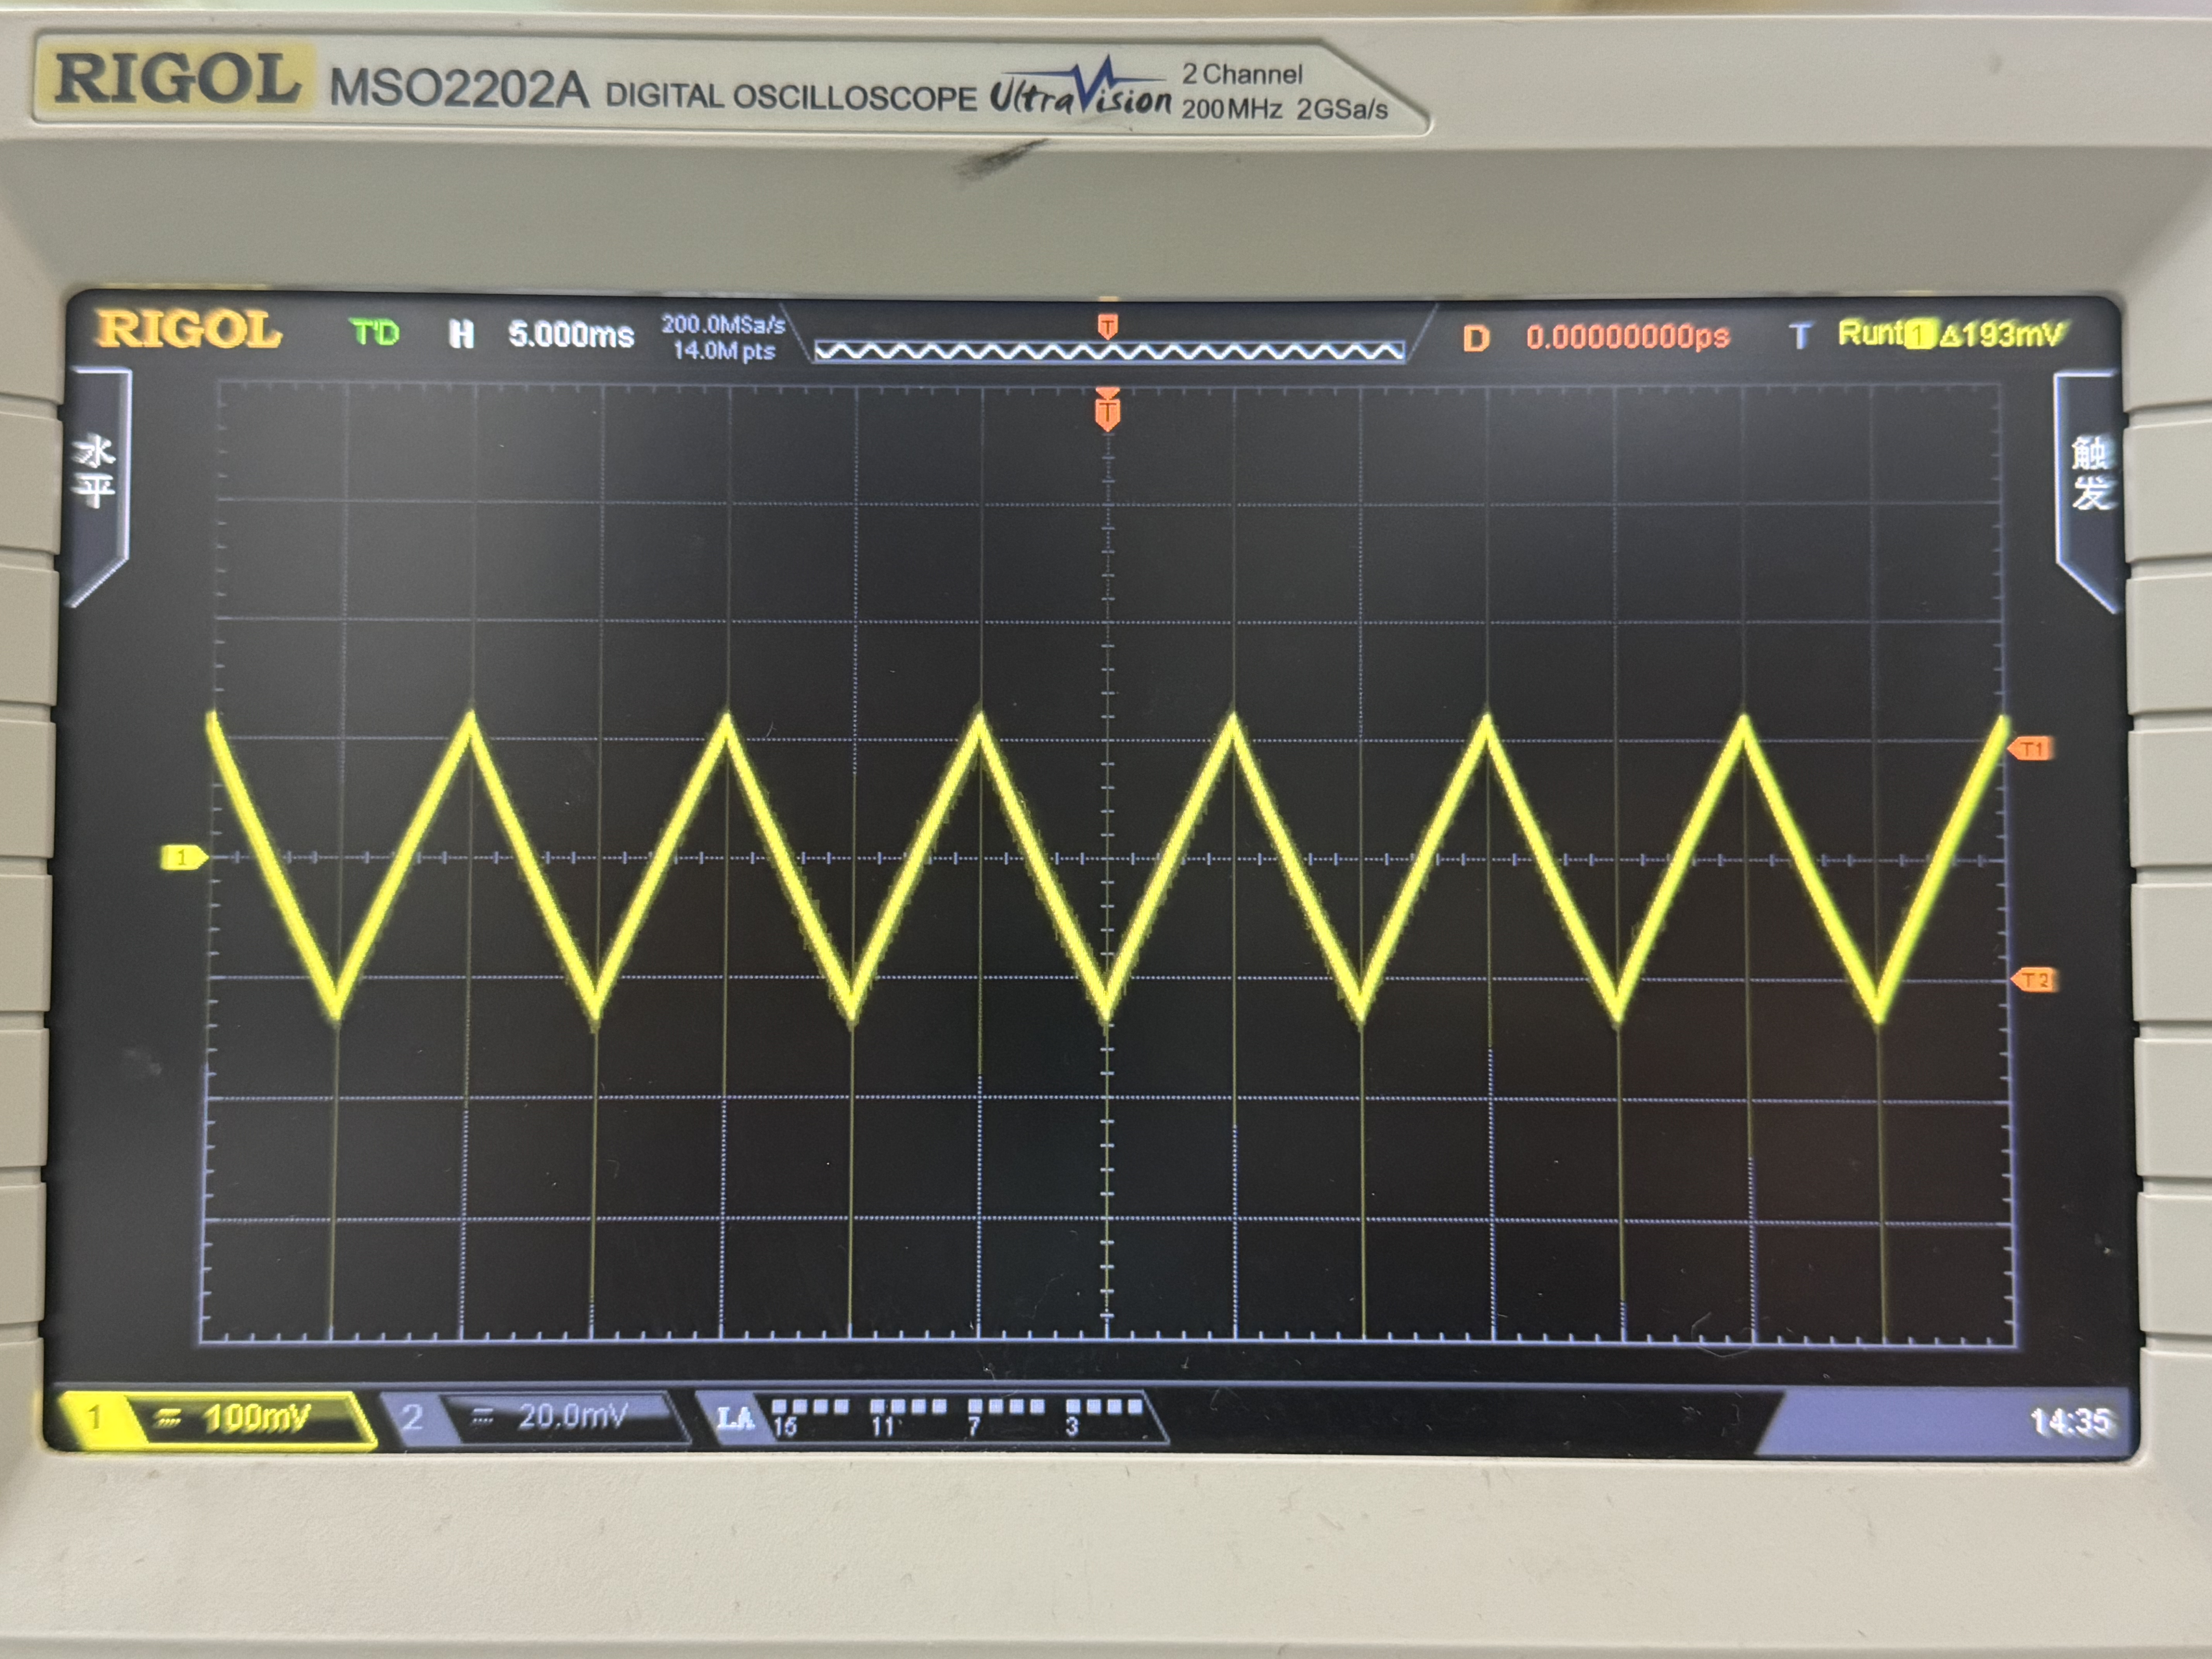
\includegraphics[width=0.4\textwidth]{rc_i2.jpg}}
            \caption{RC 积分波形图}
        \end{figure}
    \subsubsection{RL 积分电路}
        RL 微分电路如图~\ref{fig:4b} 所示,调节方波仪输出频率,使方波脉冲宽度满足微分电路的必要条件,将 $R_2$、$R_4$ 分别接入,观察微分电路输出有何不同,并将波形画在附表中。
        \begin{figure}[!ht]
            \subfloat[$R_2$\label{fig:rli1}]{\includegraphics[width=0.4\textwidth]{rl_i1.jpg}}\hspace{6mm}
            \subfloat[$R_4$\label{fig:rli2}]{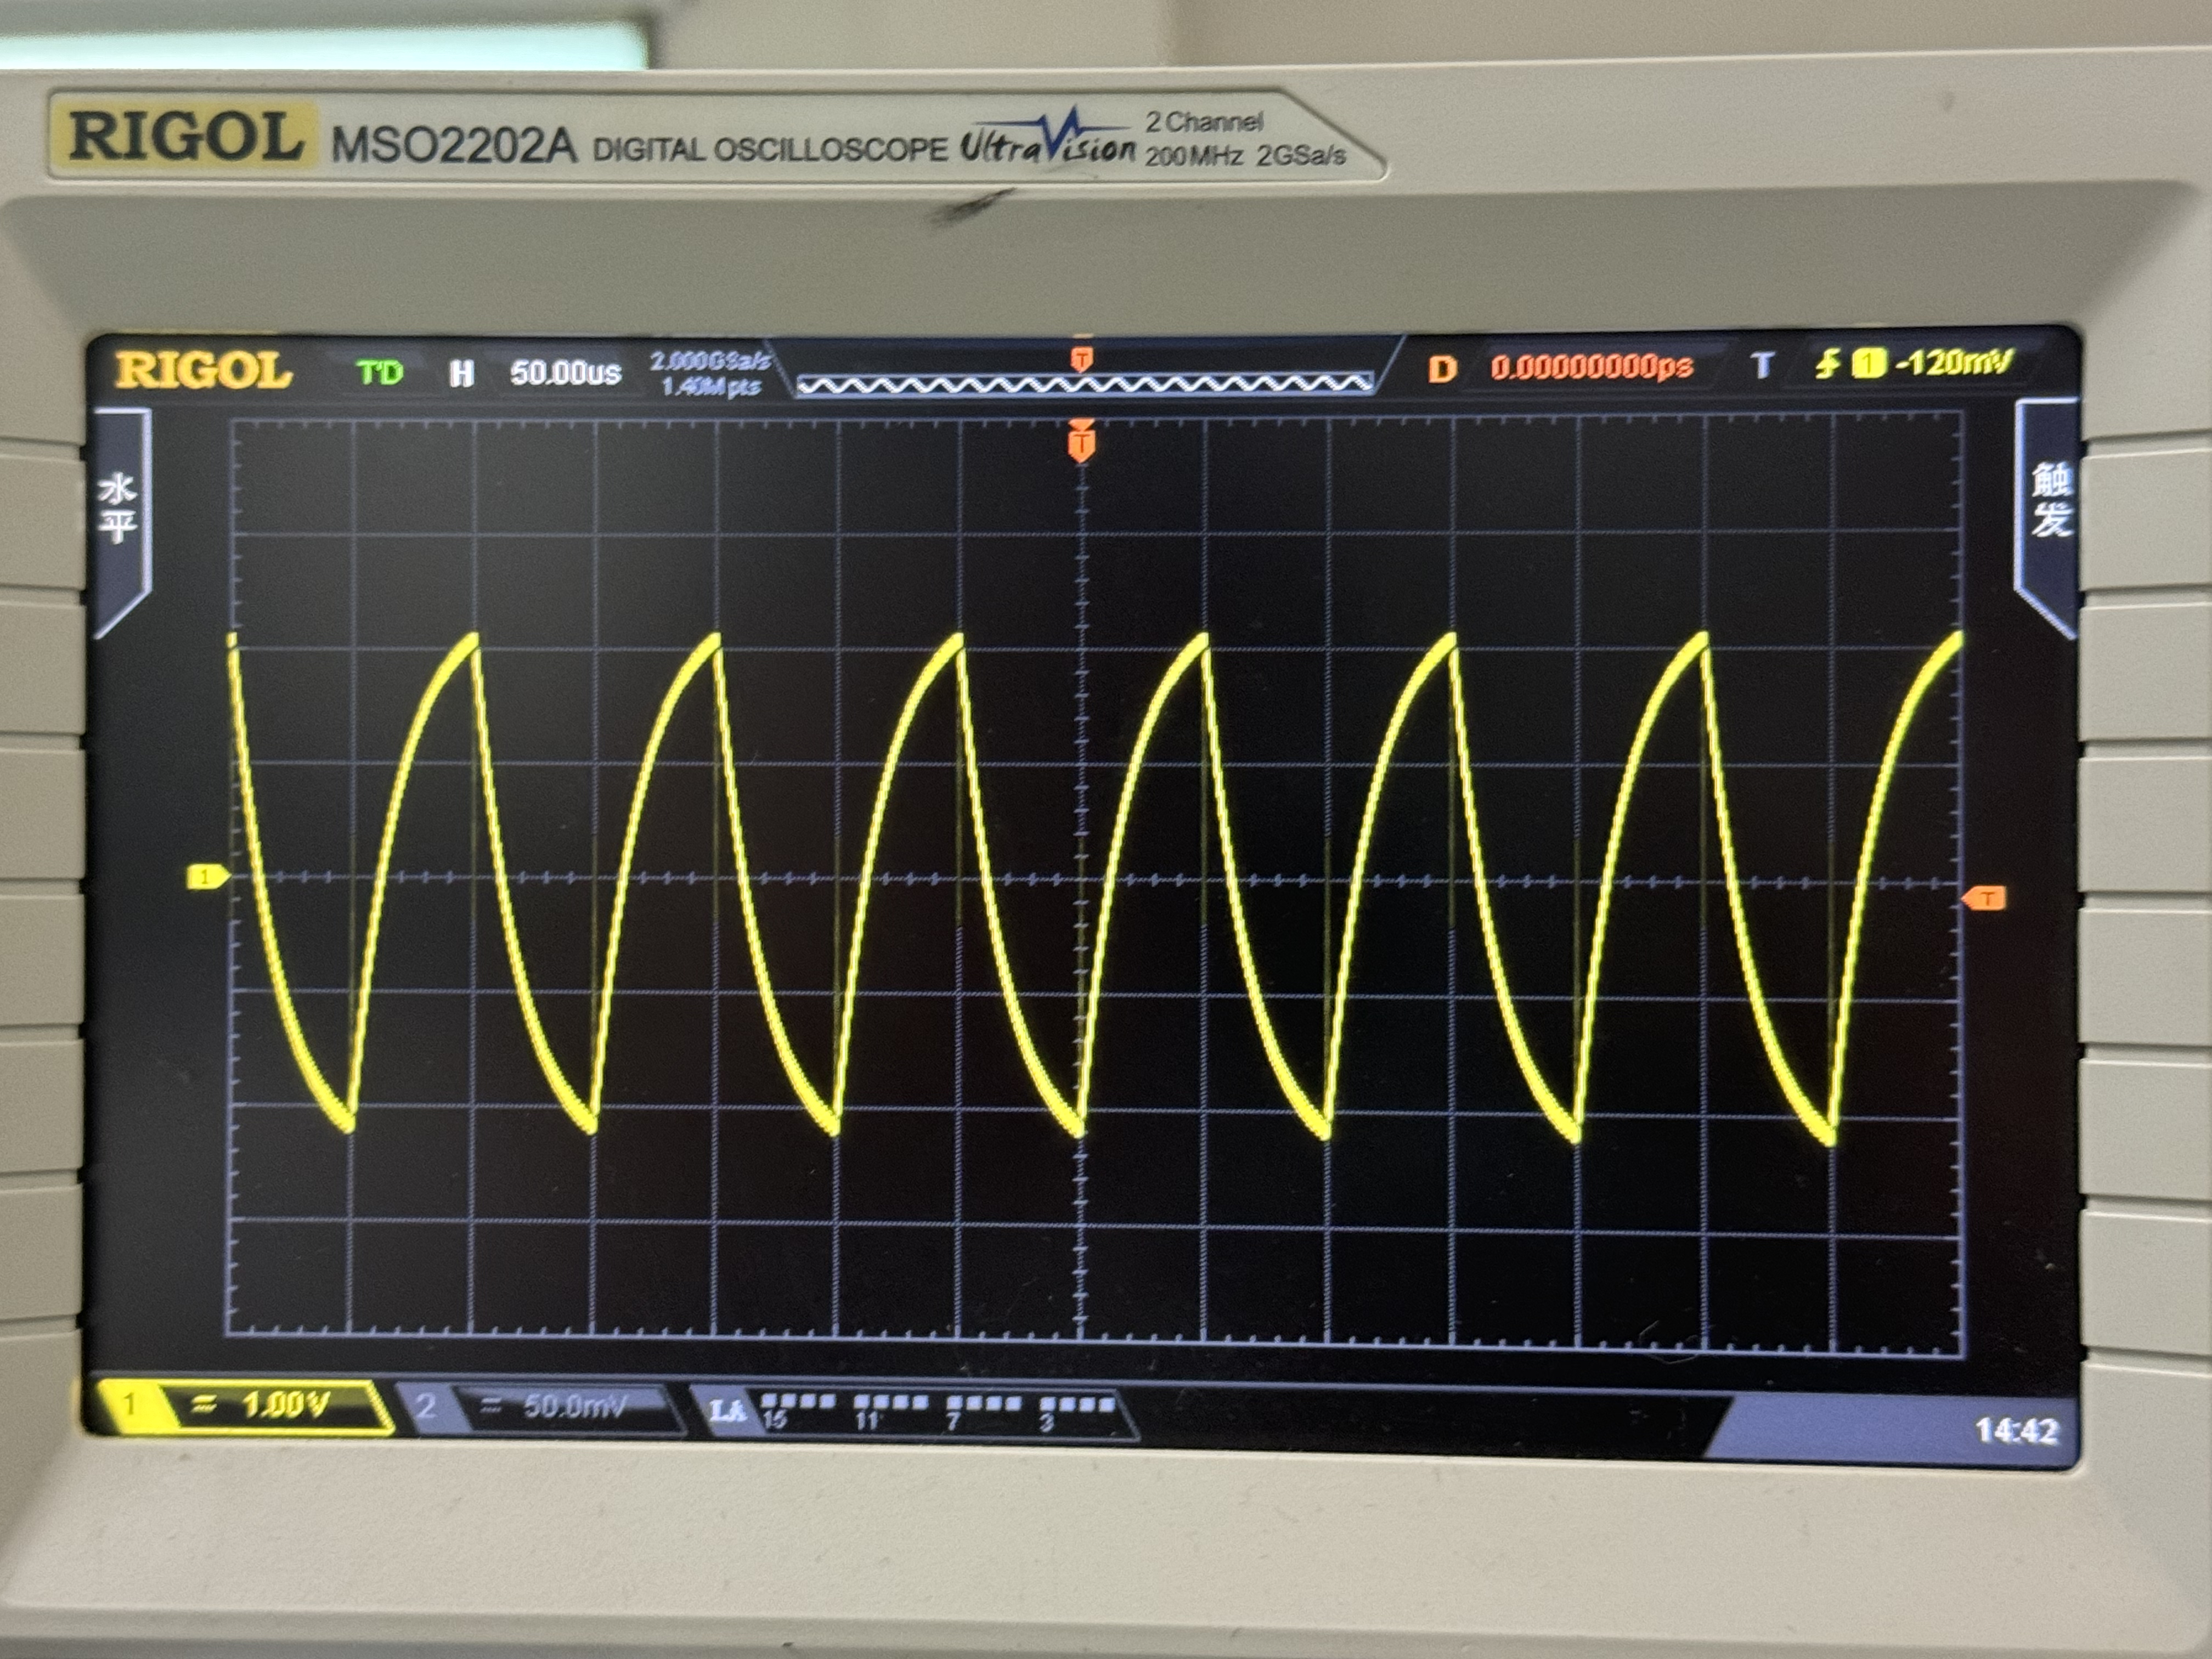
\includegraphics[width=0.4\textwidth]{rl_i2.jpg}}
            \caption{RL 积分波形图}
        \end{figure}

\section{实验分析}
\subsection{分析}
    观察前面的波形可以看出,时间常数小的电路波形较陡,时间常数大的电路波形较缓。表~\ref{tab:tau} 是各个电路的时间常数。
    \begin{table}[!ht]
        \begin{tabularx}{\textwidth}{CC *{2}{S[table-format=9.8]}} \toprule
            电路 & 接入电阻 & {理论值} & {实际值} \\ \midrule
            \multirow{2}*{RC 微分电路(\unit{\us})} & $R_2$ & 510 & 508 \\
            & $R_4$ & 240 & 244 \\
            \multirow{2}*{RL 微分电路(\unit{\us})} & $R_1$ & 33.3 & 29.4 \\
            & $R_3$ & 19.6 & 17.2 \\
            \multirow{2}*{RC 积分电路(\unit{\ms})} & $R_1$ & 30 & 32 \\
            & $R_3$ & 51.0 & 54.4 \\
            \multirow{2}*{RL 积分电路(\unit{\us})} & $R_2$ & 41.67 & 41.80 \\
            & $R_4$ & 19.61 & 19.80 \\ \bottomrule
        \end{tabularx}
        \caption{各电路时间常数\label{tab:tau}}
    \end{table}
\subsection{误差分析}
    \begin{enumerate}
        \item 温度、湿度等环境因素也会对测量结果产生影响。
        \item 元件长时间摆放导致内部结构发生变化,导致实际值发生变化。
        \item 示波器接入原电路后会对原电路的结构有一定影响,导致测量结果不准确。
    \end{enumerate}
\section{思考题}
    时间常数 $\tau = RC = \SI{5.1d-4}{\s}$,根据实验原理,方波脉宽应当是时间常数的 20 倍以上,故 $T_\text{p} \geq \SI{1.02d-2}{\s}$,即 $f \leq \SI{98}{\Hz}$
\section{实验心得}
此次实验观察到了一阶电路的动态过程。在实际操作中,观察到了由于仪器误差和连接线电阻带来的微小偏差,但总体上实验结果符合理论预期。这使得我对动态电路又有了更加清晰明确的认知。
\clearpage
\section{原始数据}
\begin{center}
    \framebox{\rotatebox{-90}{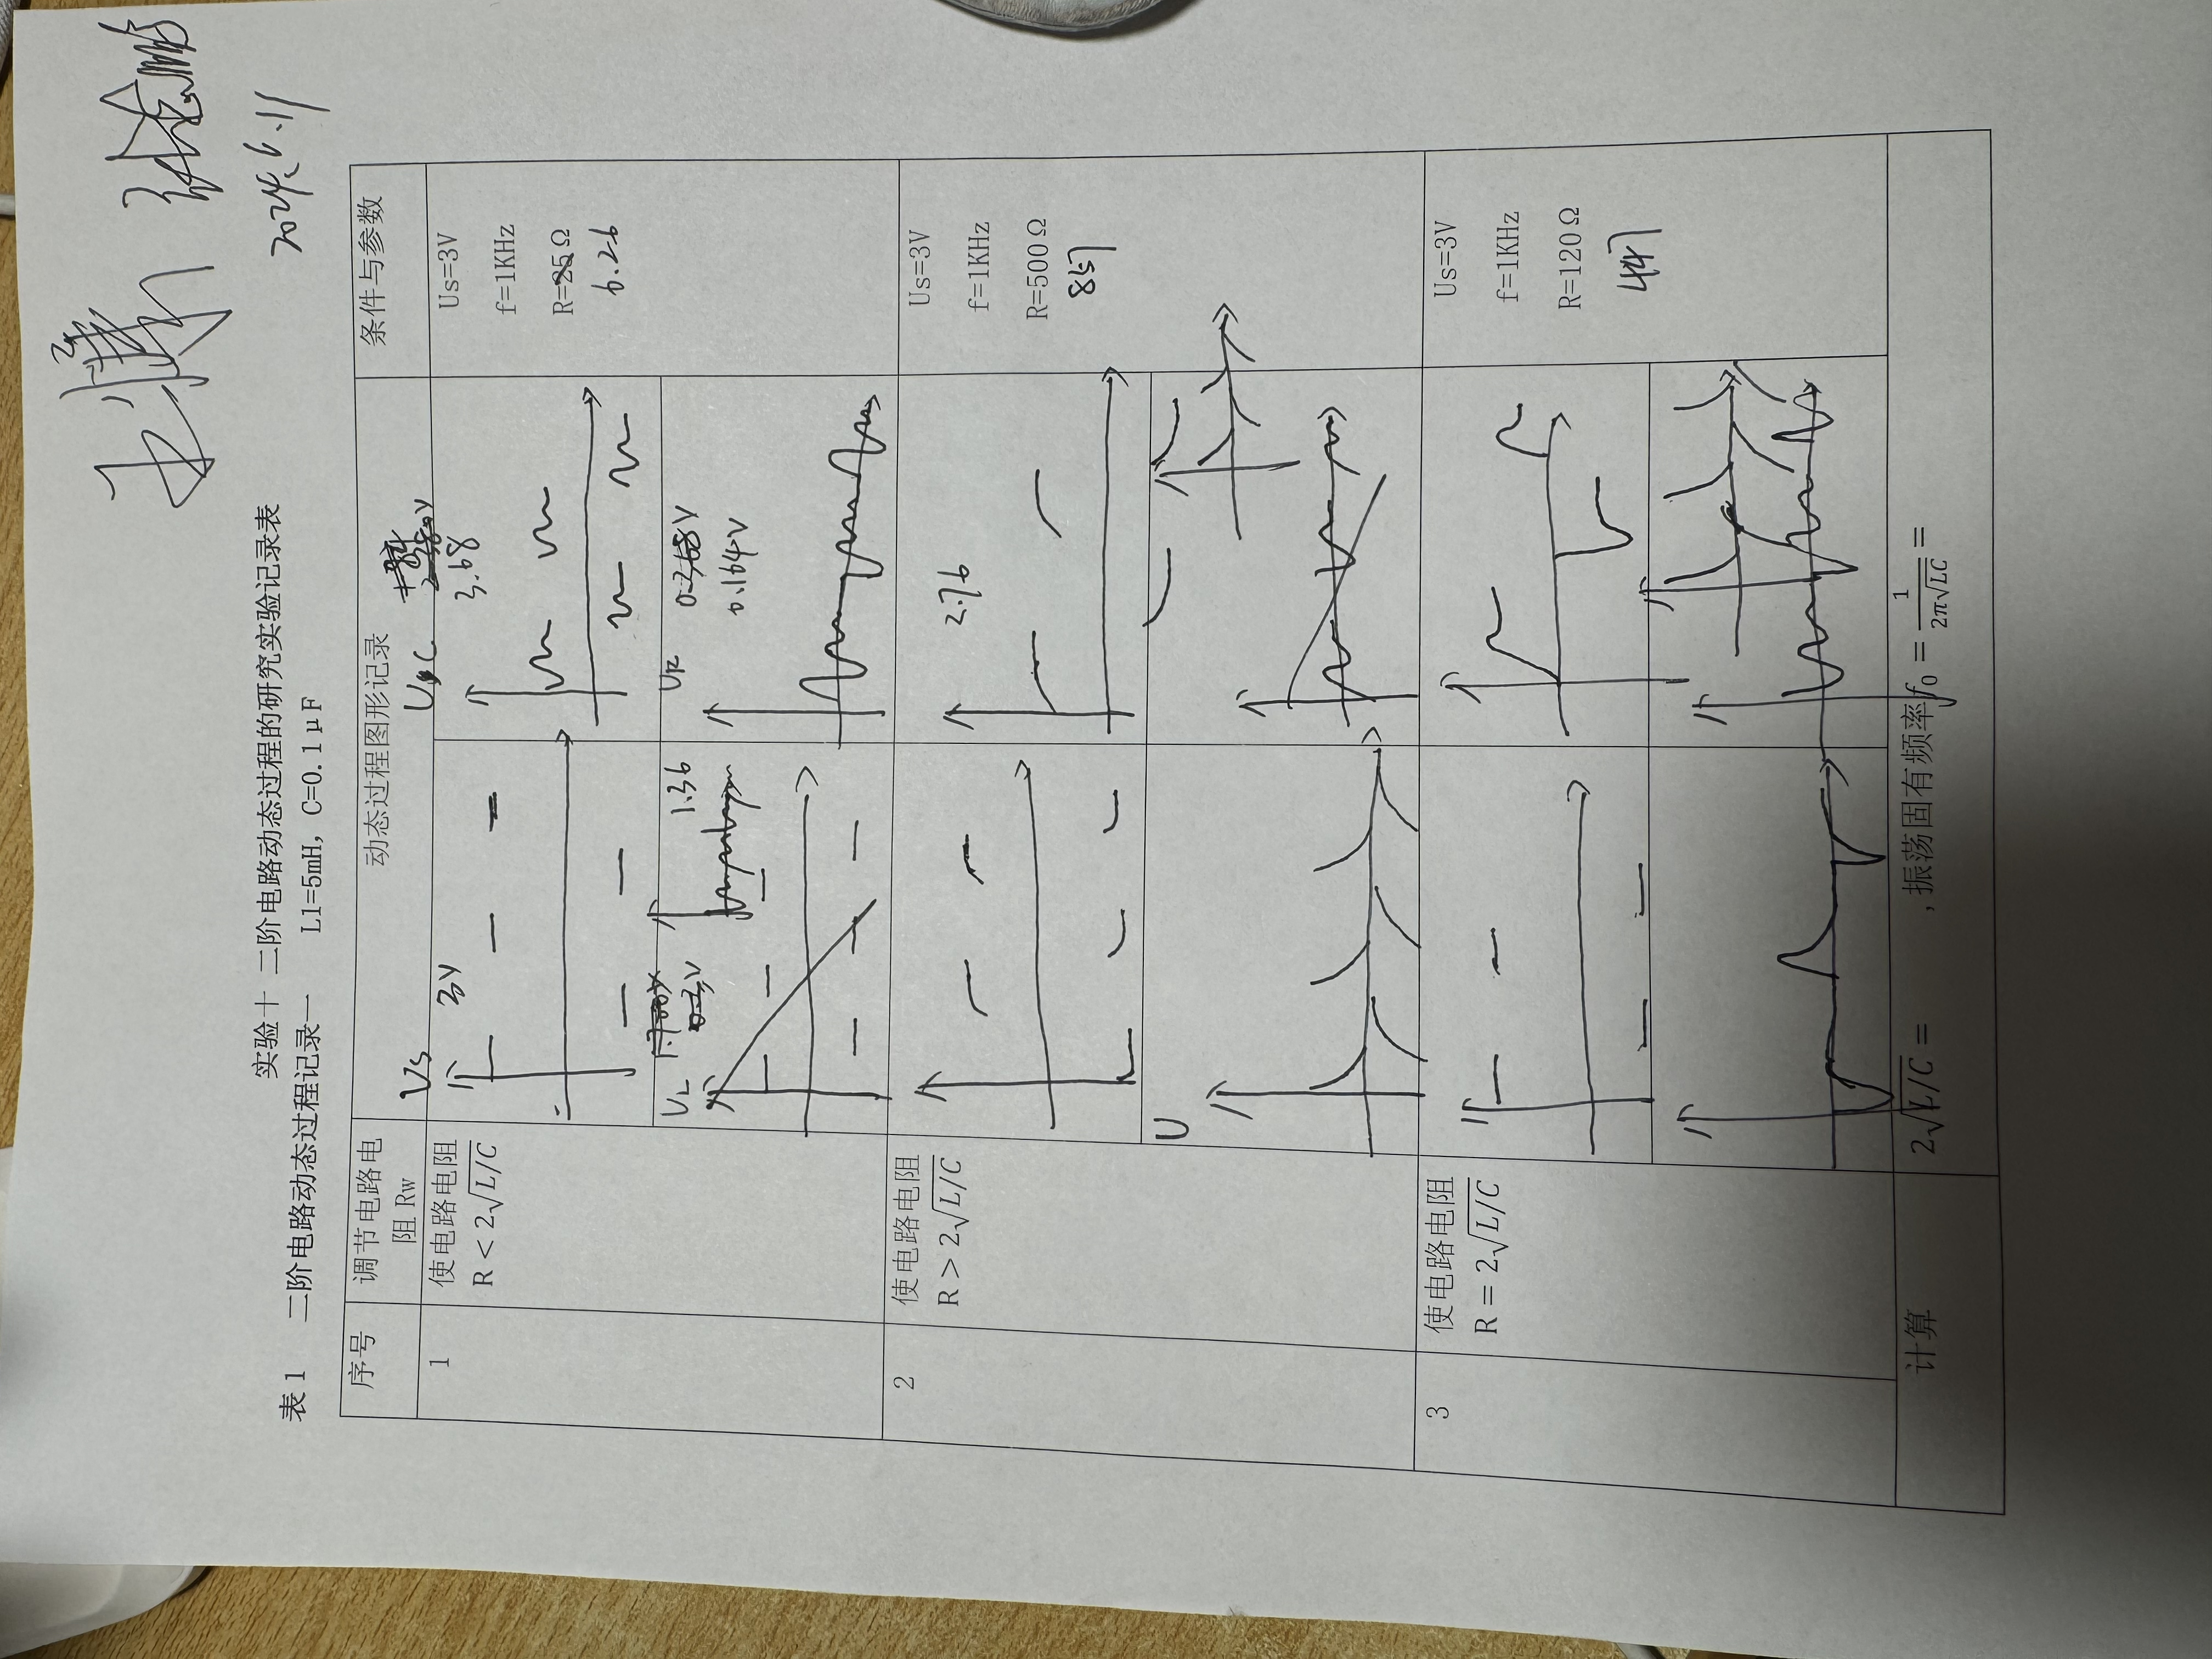
\includegraphics[height=0.95\textwidth]{rawdata.jpg}}}
\end{center}
\begin{center}
    \framebox{\rotatebox{-90}{\includegraphics[height=0.95\textwidth]{rawdata2.jpg}}}
\end{center}
\end{document}